\documentclass[UTF8,a4paper,11pt]{ctexart}
\usepackage[a4paper,margin=2.0cm]{geometry}
\usepackage{fontspec}
\usepackage{amsmath,amssymb,booktabs,multirow,graphicx,xcolor,hyperref,array}
\usepackage{caption}
\usepackage{float}
\usepackage{tikz}
\usetikzlibrary{arrows.meta,positioning,fit,calc,backgrounds}
\usepackage{fancyhdr}
\usepackage{enumitem}
\setlength{\headheight}{15pt}
\setlist{nosep,leftmargin=2em}
% 将 Markdown 风格反引号转换为等宽文本，并保护文件名中的下划线。
\catcode`\`=\active
\def`#1`{\texttt{\detokenize{#1}}}
\graphicspath{{../reports/model_strategy_ablation/m1_by_size/figures/}{../benchmarks/analysis/performance/figures/}}
\hypersetup{colorlinks=true,linkcolor=blue,urlcolor=blue,citecolor=blue}
% 图注独立于正文排版，便于快速辨识编号与说明。
\renewcommand{\figurename}{Figure}
\captionsetup[figure]{font=small,labelfont=bf,labelsep=period,
  justification=raggedright,singlelinecheck=false,skip=6pt}
\captionsetup{hypcap=false}
% 放宽浮动体的排版边界，避免短图表被单独推到空白浮动页。
\renewcommand{\topfraction}{0.92}
\renewcommand{\bottomfraction}{0.88}
\renewcommand{\textfraction}{0.08}
\renewcommand{\floatpagefraction}{0.72}
\setlength{\textfloatsep}{12pt plus 3pt minus 3pt}
\setlength{\floatsep}{10pt plus 3pt minus 3pt}
\makeatletter
\setlength{\@fptop}{0pt}
\setlength{\@fpsep}{12pt}
\setlength{\@fpbot}{0pt plus 1fil}
\makeatother

\newcommand{\version}{v0.3--中文审阅稿}
\newcommand{\method}{M1}
\newcommand{\full}{FullSchema}
\newcommand{\schemarag}{SchemaRAG}
\pagestyle{fancy}
\fancyhf{}
\fancyhead[L]{动态 Schema 与 LLM 预处理流水线}
\fancyhead[R]{\version}
\fancyfoot[C]{\thepage}

\title{\textbf{面向文化遗产记录抽取的预算感知动态 Schema 选择与\newline LLM 预处理流水线}}
\author{作者信息待补}
\date{\version\\\today}

\begin{document}
\maketitle

\begin{center}
\small 本稿为内容审阅版本；相关工作、正式参考文献和作者信息后续补充。
\end{center}

\begin{abstract}
异构文化遗产记录的信息密度和可抽取字段并不均匀，但对每条记录使用完整 Schema
会引入大量无效字段负载。尚不清楚的是，少量监督能否在不显著损害字段级抽取质量的
情况下支持记录级 Schema 裁剪，并将负载下降传递到端到端流水线。我们利用完整 Schema
抽取产生的模型辅助银标监督，训练字段存在性和输出长度预测器，再结合字段价值先验
与调用前的估计字段成本，在记录级构造预算约束的动态 Schema。使用 100 条独立银标记录
启动训练后，在与训练和验证数据隔离的 500 条冻结评估记录上，Qwen3-8B-AWQ 模型服务在
估计字段成本容量为 200 的配置下达到 Presence Macro-F1 0.7644、Micro-F1 0.7673 和
平均总 Token 385.5。相较当前 SchemaRAG 外部适配实现的固定 Top-10 检索，本方法同时
获得更高的字段一致性与更低的平均 Token；该比较限于当前 embedding 模型和 Top-$k$ 配置。
独立的 2,000 条性能负载实验进一步表明，在使用 16 个并发消费者和
容量为 16 的有界队列时，相比完整 Schema，动态字段选择使在线流水线时间降低 48.54\%，
有效吞吐提高 94.38\%，总 Token 减少 37.44\%。这些结果表明，在当前数据、模型服务
和单进程异步流水线条件下，记录级 Schema 选择具有改善大语言模型（large language
model，LLM）预处理负载的潜力。当前结果受模型辅助银标参照和在线实验边界限制，完整生命周期
成本以及多进程或多节点扩展仍需在其他系统条件下验证。
\end{abstract}

\noindent\textbf{关键词：}文化遗产抽取；动态 Schema；大语言模型；预算约束；数据预处理；在线吞吐

\section{引言}

文化遗产数据库通常由多个来源长期汇集而成，记录之间在键名、描述长度、信息密度和
可抽取字段上存在显著差异。对每条记录发送完整 Schema 虽然简化了调用
逻辑，却会使低信息记录携带大量不会产生有效结果的字段定义，并同时增加输入 Token、
输出 Token 和在线推理时间。在可能扩展至数十万条记录的应用场景中，这种固定负载不再只是提示词
设计问题，而可能成为预处理系统的运行瓶颈；本文不对该量级的端到端性能作实证推断。

已有的结构化信息抽取方法表明，大语言模型可以按照给定 Schema 输出字段值；检索增强
方法也说明，依据输入内容缩小候选 Schema 有助于减少无关字段。然而，字段选择本身
面临一个尚未解决的权衡：选择过少可能遗漏长尾字段，选择过多则会重新引入 Schema
负载和输出开销。尤其对于缺乏大规模人工字段标注的文化遗产记录，少量由完整 Schema
抽取产生的模型辅助银标监督，能否同时预测记录所需字段和输出长度，并支持质量与负载
之间可解释的记录级取舍，仍缺乏系统验证。

本文因此检验两个相互关联但需要分开回答的问题：第一，基于少量模型辅助银标监督的
字段选择器，能否在调用前根据字段存在性、预期输出长度和任务价值构造有效的动态
Schema；第二，这种字段级裁剪产生的负载变化，能否在包含排队、请求、重试和结果写入
的端到端流水线中转化为更低的运行时间和更高的有效吞吐。这里的预算是字段组合阶段
的估计容量，而不是最终 API Token 上限或货币成本上限，因此两个问题分别对应字段级
质量和系统级效率，不能由单一覆盖率或 Token 指标替代。

为回答上述问题，我们将记录级字段选择建模为预算优化。具体而言，使用字符级和词级
TF--IDF 特征预测字段存在性与输出长度，再结合字段价值先验、估计字段成本和必选字段
约束生成记录级 Schema。我们通过训练规模、预测器策略和预算策略消融，检验少量监督的
适用边界；同时与完整 Schema、仅依赖提示词的基线、固定字段策略以及基于 embedding
的动态 Schema 检索外部重实现进行对照。最后，在独立的 2,000 条性能负载上，使用单
进程异步有界 Producer--Consumer 流水线测量 Token、端到端完成时间（makespan）、有效
吞吐和尾延迟。该设计使
我们能够区分“选择器是否选得合理”和“裁剪后的负载是否改善系统运行”这两个层次的
证据。本文还对已测得的启动与初始化成本进行边界分析和敏感性检验，但多进程、多节点
扩展以及完整生命周期成本审计仍不在本文的推断范围内。

\section{问题定义与总体流程}

设原始记录为 $r$，候选字段集合为 $F$，字段选择结果为 $S_r\subseteq F$。对字段
$f$，选择器预测其存在性分数 $p(r,f)$ 和输出 Token 数 $\hat{o}(r,f)$。字段价值
权重 $w_f$ 是任务相关先验，字段定义成本为 $d_f$。动态选择写为：
\begin{equation}
 u(r,f)=p(r,f)w_f,
 \qquad c(r,f)=d_f+\hat{o}(r,f),
 \label{eq:utility-cost}
\end{equation}
\begin{equation}
 \max_{S_r}\sum_{f\in S_r}u(r,f),
 \quad \text{s.t.}\quad \sum_{f\in S_r}c(r,f)\leq B.
\end{equation}

其中 $B$ 是字段选择阶段的估计字段成本容量，并不是 LLM 调用的端到端 Token 上限，
也不是货币成本上限。换言之，`budget-200` 表示选择器尝试在估计字段成本容量 200
内组合字段，而不是限制最终请求只能产生 200 个 Token。真实调用还包括原文输入、
固定 Prompt、实际输出和重试消耗，因此最终实测 Token 高于 200 并不表示预算失效。

系统流程如下：
\begin{enumerate}
  \item Producer 从数据库读取原始记录，稳定序列化为文本；
  \item M1 预测每个字段的存在性和输出长度；
  \item 预算选择器利用字段权重和成本生成目标字段集合；
  \item Prompt 构造器生成记录级动态 Schema；
  \item Consumer 通过有界队列并发调用 LLM，执行解析、字段校验和有限重试；
  \item Writer 追加保存 JSONL 结果、Token、延迟、队列等待和错误状态。
\end{enumerate}

\begin{figure}[!ht]
\centering
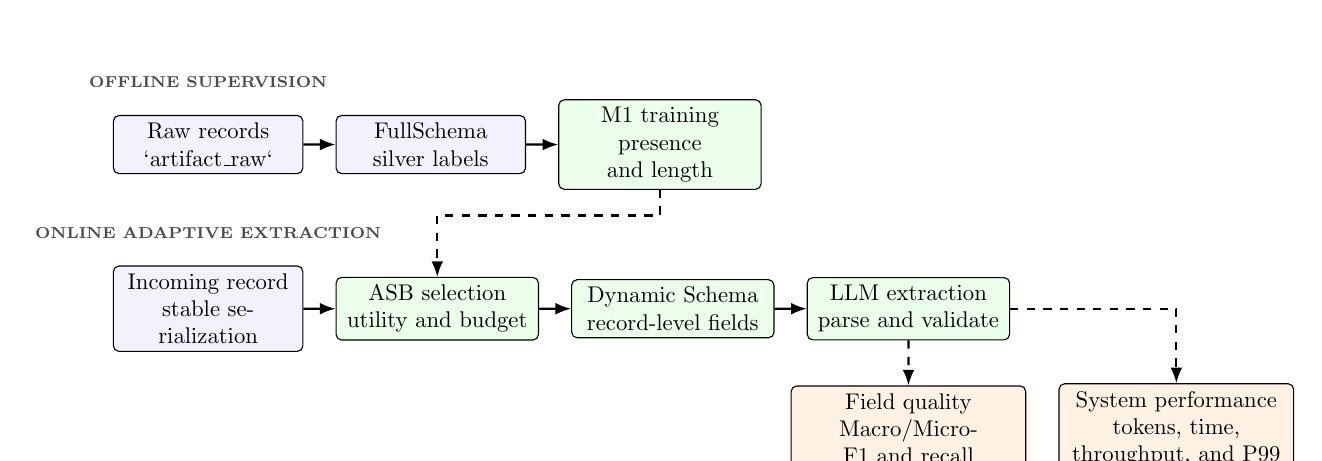
\begin{tikzpicture}[scale=0.82,transform shape,
  node distance=5mm and 5mm,
  data/.style={draw, rounded corners=2pt, align=center, minimum height=9mm,
    text width=27mm, fill=blue!5},
  process/.style={draw, rounded corners=2pt, align=center, minimum height=9mm,
    text width=29mm, fill=green!8},
  eval/.style={draw, rounded corners=2pt, align=center, minimum height=9mm,
    text width=34mm, fill=orange!10},
  stage/.style={font=\bfseries\scriptsize, text=black!70},
  arrow/.style={-{Latex[length=2mm]}, thick},
  dependency/.style={-{Latex[length=2mm]}, thick, dashed},
  evalarrow/.style={-{Latex[length=2mm]}, thick, dashed}
]
\node[stage] (offline-title) {OFFLINE SUPERVISION};
\node[data, below=3mm of offline-title] (raw) {Raw records\\`artifact\_raw`};
\node[data, right=of raw] (silver) {FullSchema\\silver labels};
\node[process, right=of silver] (train) {M1 training\\presence and length};
\draw[arrow] (raw) -- (silver);
\draw[arrow] (silver) -- (train);

\node[stage, below=7mm of raw] (online-title) {ONLINE ADAPTIVE EXTRACTION};
\node[data, below=3mm of online-title] (record) {Incoming record\\stable serialization};
\node[process, right=of record] (select) {ASB selection\\utility and budget};
\node[process, right=of select] (schema) {Dynamic Schema\\record-level fields};
\node[process, right=of schema] (llm) {LLM extraction\\parse and validate};
\draw[dependency] (train.south) -- ++(0,-4mm) -| (select.north);
\draw[arrow] (record) -- (select);
\draw[arrow] (select) -- (schema);
\draw[arrow] (schema) -- (llm);

\node[eval, below=7mm of llm] (quality) {Field quality\\Macro/Micro-F1 and recall};
\node[eval, right=of quality] (performance) {System performance\\tokens, time, throughput, and P99};
\draw[evalarrow] (llm.south) -- (quality.north);
\draw[evalarrow] (llm.east) -| (performance.north);
\end{tikzpicture}
\caption{Overall study design. Raw records construct FullSchema silver-label supervision for M1
training. The online path applies ASB selection before dynamic-Schema extraction. Field-quality and
system-performance evaluations use distinct workloads; silver labels support method development and
presence evaluation, but do not constitute an independent human Gold reference.}
\label{fig:overall-framework}
\end{figure}

\section{数据与监督信号}

项目数据库中的原始记录表 `artifact_raw` 与已有的完整抽取结果表 `artifact_extract` 通过
记录标识字段 `artifact_id` 对齐。`artifact_id` 是一条文化遗产记录的唯一标识，仅用于
跨表连接、数据划分和跨批次结果配对，不作为模型输入特征。内连接得到 6,763 条记录；本实验的
候选字段集合 $F$ 包含 18 个预先定义的目标抽取字段，而非原始 JSON 中任意可见的键。数据划分为训练集
5,410 条、验证集 677 条和测试集 676 条。
`gold_main` 为测试集中的 500 条冻结子集，不与训练集或验证集重叠。

表~\ref{tab:field-schema}给出候选字段的语义角色、预设任务权重和训练集中的银标非空率。字段权重
是任务配置中的价值先验，并非从当前数据学习得到；`name` 与 `category` 为必选字段，始终被
保留在动态 Schema 中。其余字段由选择器在每条记录上决定是否纳入。FullSchema 指包含 $F$ 全部
字段的固定抽取配置；动态 Schema 则是针对记录 $r$ 选出的子集 $S_r\subseteq F$。因此，字段选择
的最小单位是目标抽取字段，而不是原始记录的任意 JSON 键。

\begin{table}[htbp]
\centering
\footnotesize
\caption{Candidate extraction fields and their roles in the cultural-heritage Schema. Prevalence is the
non-empty rate of the FullSchema-derived silver reference in the 5,410-record training split. Weights are
pre-specified task values rather than estimates learned from this dataset.}
\label{tab:field-schema}
\begin{tabular}{@{}>{\raggedright\arraybackslash}p{.25\textwidth}>{\raggedright\arraybackslash}p{.24\textwidth}c c>{\raggedright\arraybackslash}p{.20\textwidth}@{}}
\toprule
Fields & Semantic role & Weight & Required & Training prevalence \\
\midrule
`name`, `category` & Object identity and category & 1.0, 0.9 & Yes & 100.0\%, 100.0\% \\
`form_type`, `material`, `period` & Form, material, and dating & 0.9, 0.9, 0.8 & No & 98.8\%, 99.7\%, 99.8\% \\
`dynasty`, `usage` & Historical attribution and function & 0.9, 0.7 & No & 74.8\%, 63.3\% \\
`motif`, `related_person`, `culture` & Decoration, related person, and cultural attribution & 0.7, 0.5, 0.6 & No & 23.9\%, 13.8\%, 6.9\% \\
`region`, `craft_school`, `acq_type` & Provenance region, production school, and acquisition & 0.6, 0.6, 0.4 & No & 3.5\%, 1.8\%, 1.6\% \\
`condition`, `site`, `related_event`, `craft` & Condition, site, related event, and technique & 0.6, 0.6, 0.4, 0.6 & No & 0.9\%, 0.8\%, 0.6\%, 0.5\% \\
`desc` & Narrative description & 0.5 & No & 100.0\% \\
\bottomrule
\end{tabular}
\end{table}

`artifact_extract` 不是人工真值。它是既有 FullSchema 过程产生的 model-assisted
silver reference。对字段 $f$，非空 FullSchema 输出构造 `present=1`，空值构造
`present=0`；非空字段值使用 `cl100k_base` 统计 Token 数作为长度标签。因此模型
学到的是 FullSchema 输出行为，而非已被独立人工确认的事实真实性。该边界同时适用于
第一部分离线评估和 `gold_main` 的字段存在性评价。

本文的 Presence 指标把每个候选字段的非空/空值判断视为一个二分类任务。对每个字段
分别计算 $F1_f$ 后取算术平均得到 Presence Macro-F1；将所有字段和记录的决策汇总后
计算 TP、FP、FN，再得到 Presence Micro-F1。前者让稀有字段与高频字段等权，后者按
字段实例加权，因此二者差距可以反映类别不均衡。Exact Value Recall 则只在参考值和
预测值均存在时比较完整值是否一致，并以参考非空字段为分母；Coverage 只表示输出中
非空字段相对于参考非空字段的比例，不等同于值正确率。Length MAE 仅评价银标非空
字段的输出长度预测误差，不能解释为真实 API Token 误差。

训练规模消融使用 50、100、250、500、1000、2500 和 5410 条，每个规模使用 5 个
seed。本文将 $n$ 定义为用于训练 M1 的 FullSchema 银标记录数；它不是测试记录数，
也不是单次 LLM 请求的字段数。seed 是控制训练初始化、数据顺序和抽样过程的随机种子，
用于检查结果是否依赖某一次随机运行。固定 seed 下采用多标签缺口贪心顺序构造嵌套训练
前缀，因此小规模样本是大规模样本的前缀，不应视为完全独立的均匀抽样。后文的“100 条
银标启动样本三种子主结果”特指稳定版 Prompt 下三个随机种子的真实 LLM 对照，不与本节
表格中的五个随机种子离线模型消融混用。

\section{方法实现}

\subsection{基于稀疏文本特征的字段预测器}

\subsubsection{输入、标签与监督目标}

对每条原始记录 $r$，系统将其 JSON 键值及描述文本稳定序列化为 `record_text`；同一条
记录的字符级与词级特征向量由该文本共同构成，并供所有候选字段共享使用。字段 $f$ 的
存在性标签定义为 $y_f(r)\in\{0,1\}$：FullSchema 银标中该字段非空时为 1，空值时为 0。
仅当 $y_f(r)=1$ 时，才以该字段值经 `cl100k_base` 编码得到的 Token 数 $o_f(r)$ 作为长度
监督。训练、验证和测试记录按 `artifact_id` 划分且互不重叠；验证集只用于字段阈值校准，
测试集不参与任一训练或校准步骤。因而 M1 预测的是完整 Schema 抽取的银标行为，
而不是经人工独立确认的字段事实。

\subsubsection{共同训练协议与训练规模设计}

三种模型均对 18 个候选字段逐字段训练存在性分类器，而不是训练一个共享的多标签输出层；
每个分类器均采用 `class_weight=balanced`、`liblinear` 求解器、最多 1,000 次迭代，并以当前
随机种子初始化。所有 TF--IDF 词表和 IDF 权重仅在对应训练子集拟合，再变换验证集和测试集，
从而避免记录文本或测试字段频率泄漏到模型选择过程。长度预测在字段训练正样本少于 10 条时
回退为训练正样本长度中位数；其余情况使用 Ridge 回归（$\alpha=10$）拟合
$\log(1+o_f(r))$。因此，分类和长度分支的比较保持相同的标签、划分和回退规则。

训练规模实验使用 $n\in\{50,100,250,500,1000,2500,5410\}$，并在五个固定随机种子
（42--46）下重复。每个较小规模训练集是同一 seed 对应较大规模训练集的嵌套前缀；前缀由
多标签缺口贪心排序构造，以尽可能维持各字段的正例比例。这一设计使规模曲线比较的是监督量，
而非彼此无关的抽样波动。Character、M1 和 M2 均在全部训练规模上测量，因此图~\ref{fig:offline-main}
可以直接比较三种特征融合策略随监督规模变化的趋势。M2 仍仅用于离线消融，不进入在线 ASB 或真实
LLM 抽取实验。

\subsubsection{Character TF--IDF 基线}

最初的字符级基线仅使用字符级 TF--IDF（2--5 gram）表示 `record_text`。其最小文档频数为 2，
特征上限为 100,000，并采用次线性词频缩放。对每个候选字段独立训练分类器，
并在验证集按 F1 最大化选择原始阈值。该设计保留字段键名、简称、编号和局部格式等字符模式，
而不依赖中文分词；它是后续融合模型的共同参照，而非在线 ASB 的最终字段选择器。其长度分支
遵循共同训练协议，并预测银标输出长度。

\subsubsection{M1：早融合字段预测器}

M1 将字符级 TF--IDF（2--5 gram，`min_df=1`，最多 100,000 个特征）和词级 TF--IDF
（1--2 gram，`min_df=1`，最多 50,000 个特征）拼接为一个稀疏矩阵；两者均采用
`sublinear_tf=True`。词级分析使用 sklearn 默认的 token 规则，而非显式中文分词。对每个字段
分别训练分类器，输出存在性分数 $p(r,f)$。用于离线二分类评价的字段阈值先在验证集按 F1 最大化
选择，再向 0.5 收缩 25\%，并限制在 0.10--0.90，以避免小验证集上的极端阈值直接迁移到测试集。
长度预测遵循共同协议；推理时先作指数逆变换，再四舍五入并截断为非负整数，得到
$\hat{o}(r,f)$。

训练集中始终非空的 `name`、`category` 和 `desc` 使用常量预测；这些字段的高 F1 不代表
模型学到了可迁移的区分能力。相反，`craft`、`site`、`acq_type`、`craft_school` 和
`related_event` 等长尾字段的正样本不足，是 M1 宏平均表现的主要限制。存在性概率与长度
估计分别刻画了“该字段可能有值”和“该字段可能带来的输出负载”，二者不应被解释为字段值
正确性或真实 API Token 的直接预测。

\subsubsection{M2：后融合消融模型}

M2 使用与 M1 相同的字符级和词级 TF--IDF 配置，但不在特征层拼接。对每个字段，它分别训练
字符模型和词模型，枚举验证集的 $\alpha\in\{0,0.25,0.5,0.75,1\}$，并以融合后 F1 最大为准
选择字段特异的融合权重及阈值；F1 相同时优先选择更接近 0.5 的权重：
\begin{equation}
p_{\mathrm{M2}}(r,f)=\alpha p_{\mathrm{char}}(r,f)+(1-\alpha)p_{\mathrm{word}}(r,f).
\end{equation}
选出的阈值同样向 0.5 收缩 25\% 并限制在 0.10--0.90。长度分支仍采用拼接特征，与 M1 完全
一致。因此，M2 只检验存在性概率的融合位置；它仅用于离线消融，在当前实现中不进入 ASB，也
不参与真实 LLM 抽取实验。

\subsubsection{与预算选择器的接口及边界}

M1 在 LLM 调用前运行，但不生成最终字段值，也不直接决定动态 Schema。其输出
$p(r,f)$ 与 $\hat{o}(r,f)$ 分别输入式（\ref{eq:utility-cost}）中的字段效用和估计成本，
随后由必选字段约束与 0--1 背包选择器产生 $S_r$。采用 TF--IDF 与线性模型的目的，是在少量
银标启动样本下提供低延迟、可检查的字段裁剪信号，而非获得深层语义表示。预算选择限制的
仍是调用前字段组合的估计容量；完整 Prompt、原始记录、模型实际输出和重试引起的最终
Token 消耗由在线实验单独测量。

\begin{center}
\centering
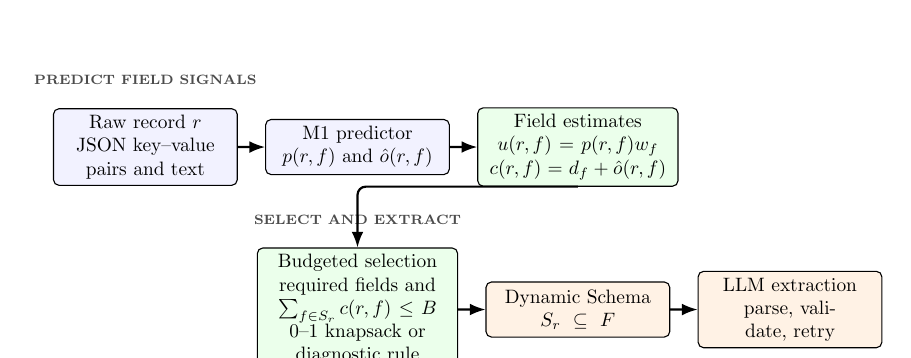
\begin{tikzpicture}[scale=0.70,transform shape,
  node distance=5mm and 5mm,
  input/.style={draw, rounded corners=2pt, align=center, minimum height=10mm,
    text width=31mm, fill=blue!5},
  decision/.style={draw, rounded corners=2pt, align=center, minimum height=10mm,
    text width=34mm, fill=green!8},
  output/.style={draw, rounded corners=2pt, align=center, minimum height=10mm,
    text width=31mm, fill=orange!10},
  arrow/.style={-{Latex[length=2mm]}, thick},
  stage/.style={font=\bfseries\scriptsize, text=black!70}
]
\node[stage] (predict-title) {PREDICT FIELD SIGNALS};
\node[input, below=3mm of predict-title] (record) {Raw record $r$\\JSON key--value pairs and text};
\node[input, right=of record] (m1) {M1 predictor\\$p(r,f)$ and $\hat{o}(r,f)$};
\node[decision, right=of m1] (score) {Field estimates\\$u(r,f)=p(r,f)w_f$\\$c(r,f)=d_f+\hat{o}(r,f)$};
\draw[arrow] (record) -- (m1);
\draw[arrow] (m1) -- (score);
\node[stage, below=6mm of m1] (select-title) {SELECT AND EXTRACT};
\node[decision, below=3mm of select-title] (select) {Budgeted selection\\required fields and $\sum_{f\in S_r}c(r,f)\leq B$\\0--1 knapsack or diagnostic rule};
\node[output, right=of select] (schema) {Dynamic Schema\\$S_r\subseteq F$};
\node[output, right=of schema] (llm) {LLM extraction\\parse, validate, retry};
\draw[arrow, rounded corners=3pt] (score.south) -| (select.north);
\draw[arrow] (select) -- (schema);
\draw[arrow] (schema) -- (llm);
\end{tikzpicture}
\captionof{figure}{ASB dynamic-Schema decision architecture. M1 predicts field presence and output length
from each raw record; the selector combines field value, estimated cost, and required-field constraints
to construct a record-level Schema. The SchemaRAG comparator bypasses M1 and budgeted cost, using an
independent query--field embedding Top-$k$ ranking.}
\label{fig:asb-decision}
\end{center}

\subsection{实验策略定义}

为避免把不同性质的对照混在一起，本文将策略分为完整 Schema 基线、仅依赖提示词的
基线、固定字段诊断、本方法的动态策略和外部方法五类。各策略的字段选择规则如下。

\begin{center}
\centering
\scriptsize
\renewcommand{\arraystretch}{0.88}
\captionof{table}{Inputs, selection mechanisms, and comparison roles of extraction strategies.}
\label{tab:strategies}
\begin{tabular}{>{\raggedright\arraybackslash}p{2.2cm}>{\raggedright\arraybackslash}p{3.3cm}>{\raggedright\arraybackslash}p{5.5cm}>{\raggedright\arraybackslash}p{3.4cm}}
\toprule
Strategy & Input fields & Field-selection or prompt mechanism & Comparison role\\
\midrule
`full` & All 18 fields & No pruning; base extraction prompt & Full-Schema baseline\\
`prompt-null` & All 18 fields & Output `null` without reliable evidence & Strict prompt-only baseline\\
`prompt-omit` & All 18 fields & Permit omitted fields without reliable evidence & Prompt-only output control\\
`fixed-5/10` & Fixed 5 or 10 fields & Fixed field weights; ignores the current record & Fixed-field diagnostic\\
`budget-200/400` & Record-level field subset & M1 prediction followed by a capacity-specific 0--1 knapsack & Dynamic strategy\\
`lambda` & Record-level field subset & M1 prediction followed by a net-utility threshold & No-hard-budget control\\
`SchemaRAG k=10/15` & Top-$k$ field subset & Cosine ranking of query and field vectors & External reimplementation\\
\bottomrule
\end{tabular}
\end{center}

`full` 始终向 LLM 提供本实验的 18 个候选字段，不使用 M1，是输入完整性和在线负载的
主要基线。`prompt-null` 与 `prompt-omit` 也保留完整 Schema，只改变指令：前者要求
无可靠依据时输出 `null`，后者允许省略字段。因此它们可以检验仅依靠 Prompt 是否
能够替代实际的 Schema 裁剪，但不能减少 Schema 输入负载。`fixed-5` 和 `fixed-10`
不读取当前记录内容，而是按预先固定的字段权重取字段；由于其字段集合主要包含数据
中较稠密的字段，存在先验偏置，只作为补充诊断，不参与动态方法的公平主排序。

`budget-200` 和 `budget-400` 首先由 M1 预测字段存在性分数和输出长度，再计算每个
字段的估计字段成本与任务效用，强制保留必选字段，最后用 0--1 背包在容量
200 或 400 内最大化总效用。无硬预算策略的正则化系数为 $\lambda=0.003$，使用相同的
M1 预测和字段权重，但不设硬容量，而按净收益 $u(r,f)-\lambda c(r,f)$ 选择字段，并
强制保留必选字段。对非必选字段，该规则等价于仅在
$u(r,f)/c(r,f)>\lambda$ 时选入字段；因此，$\lambda$ 是当前效用和估计成本标度下的
选择门槛，而不是 API 价格、Token 上限或货币成本。增大 $\lambda$ 会提高字段进入门槛，
通常减少选中字段和 Token；减小 $\lambda$ 则趋向保留更多字段，但不提供硬容量保证。
本文取 $\lambda=0.003$ 作为无硬预算软惩罚对照，用于观察取消硬容量后的字段覆盖与负载变化，
不将其解释为跨数据集或跨模型的最优值。

这里的估计字段成本只用于调用前决策：
\begin{equation}
 \widehat{C}_{field}(r,f)=C_{schema}(f)+\widehat{C}_{output}(r,f).
\end{equation}
它不是实际 API 成本。LLM 调用完成后，系统从 API usage 测量 `input_tokens`、
`output_tokens` 和 `total_tokens`，重试产生的 Token 也累计到任务和运行级统计中。
因此，估计成本决定“选哪些字段”，实测 Token 决定“实际消耗了多少”，两者不能互相
替代。

更完整地区分三个层次：
\begin{align}
 \widehat{C}_{field}(r,f)&=C_{schema}(f)+\widehat{C}_{output}(r,f),\\
 C_{online}(r)&=\sum_{a\in\mathrm{attempts}(r)}
               \left(C_{input,a}^{actual}+C_{output,a}^{actual}\right).
\end{align}
第一项在请求发出前可用，服务于字段选择和预算约束；第二项只能在请求结束后从
API usage 和每次尝试记录中获得，是本文比较在线效率的依据。原始记录输入通常无论
选择多少字段都需要发送，因此没有放入字段组合预算，但它计入 `C_{online}`；重试
请求也通过上式按尝试逐次计入。

\subsection{基于 Embedding 的 SchemaRAG 外部适配实现}

SchemaRAG 在本文中作为独立的语义检索式字段选择器实现，不使用 M1 的字段存在性分数、
长度预测或预算背包。它回答的是一个不同的问题：在不学习记录级字段标签的条件下，原始
记录与哪个字段描述在语义表示空间中更接近。为保证比较对象清晰，SchemaRAG 只替换
动态 Schema 的字段选择环节，所选字段随后进入与其他方法相同的下游 LLM 抽取流程。

\subsubsection{检索表示与字段排序}

对每个字段 $f$，实现分别对字段名和字段定义调用 Embedding 服务，以 0.5/0.5 加权后
进行 L2 归一化，得到字段向量 $\bar{e}(f)$。对记录 $r$，将固定检索指令与稳定序列化的
原始记录拼接为 query 文本，并用同一服务得到归一化 query 向量 $\bar{e}(r)$。字段按
余弦相似度排序：
\begin{equation}
 s(r,f)=\left\langle\bar{e}(r),\bar{e}(f)\right\rangle,
 \qquad S_r=\operatorname{TopK}_{f\in F}s(r,f).
\end{equation}
由于向量已归一化，上式的点积等价于余弦相似度。实现从 18 个候选字段中选择 Top-10
或 Top-15 字段，并以 $S_r$ 构造记录级动态 Schema：

\begin{center}
\texttt{raw record -> query embedding -> cosine ranking -> Top-k fields -> LLM}
\end{center}

\subsubsection{在线开销与统一结果接口}

当前实现使用统一实验环境提供的 `Qwen3-Embedding-0.6B`。字段向量可按 Schema、
Embedding 模型、组合权重和检索指令的配置哈希缓存；每条记录的 query embedding 则必须
在线生成，并计入端到端时间。字段向量的读取或首次构建时间以 `schema_embedding_ms`
单独记录，记录级检索时间以 `query_embedding_ms` 记录。M1 的长度预测仅在统一结果
协议中为已选字段填写
\texttt{estimated\allowbreak\_field\allowbreak\_cost}，既不参与 Top-k 排序，也不是 SchemaRAG
在线运行的必要输入。因此，实测 Token 和在线时间仍由实际 LLM 调用及检索请求记录决定，
不能以该辅助估计成本替代。

\subsubsection{适配范围与复现边界}

该方法依据 SchemaRAG 的公开方法描述完成适配，是外部独立重实现而非官方代码复现。
当前实例实现固定 Top-k 的字段检索，不包含字段分段、示例检索或二阶段重排序；因此，
它检验的是“基于 Embedding 的固定 Top-k 字段检索”在本任务中的表现，而不是完整
SchemaRAG 系统的性能上限。后文与 M1 的比较仅限于当前实现、模型服务和实验条件，
不应被解释为对官方方法的严格复现或普遍优越性结论。

\subsection{在线执行与指标实现}

当前实现是单进程异步有界 Producer--Consumer。并发参数 `c` 控制 Consumer 数量，
队列容量 `q` 控制 `asyncio.Queue` 大小；队列满时 Producer 阻塞形成背压。任务按照
输入顺序增量构造，成功任务按方法和配置哈希断点续跑，失败任务在最多两次重试后
保留错误状态。

\begin{equation}
 \mathrm{makespan}=t_{finish}-t_{start},\qquad
 \mathrm{effective\ throughput}=\frac{N_{success}}{\mathrm{makespan}}.
\end{equation}

`pipeline_ms` 的起止点覆盖在线记录读取、任务构造、入队、LLM 请求、重试和结果写入。
它不包含 100 条 FullSchema 启动样本生成、训练数据和银标标签构造、M1 离线训练、
模型或向量器加载。当前 M1 使用既有 `training_dataset.jsonl`，训练本身不调用 LLM。
因此本文系统结果是在线推理结果，不是全生命周期成本结果。选择 `budget-200` 也不是
因为它对应某个 API 的 200-token 限额，而是因为离线回放中它在容量、字段覆盖和请求
负载之间提供了中间 operating point；真实 LLM 三 seed 中它相较 `budget-400` 和
无硬容量的 lambda 对照具有更低 Token，同时字段指标没有出现明显崩溃。这个选择是
当前数据和服务条件下的工程折中，不应写成全局最优预算。

为明确在线执行边界，图~\ref{fig:online-execution} 展示单进程 Runner 的数据流。Producer
只负责读取、规划和入队；Consumer 负责请求、解析、校验和有限重试；Writer 负责持久化
结果与运行指标。有界队列是背压位置，不表示已经实现多进程或跨节点调度。

\begin{figure}[htbp]
\centering
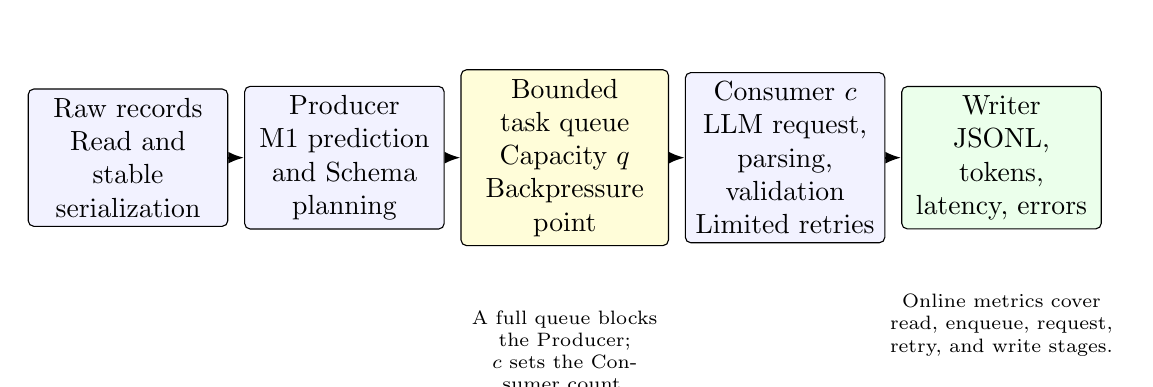
\begin{tikzpicture}[
  node distance=4mm and 2mm,
  block/.style={draw, rounded corners=2pt, align=center, minimum height=9mm,
    text width=23mm, fill=blue!5},
  queue/.style={draw, rounded corners=2pt, align=center, minimum height=12mm,
    text width=24mm, fill=yellow!15},
  output/.style={draw, rounded corners=2pt, align=center, minimum height=9mm,
    text width=23mm, fill=green!8},
  arrow/.style={-{Latex[length=2mm]}, thick},
  note/.style={font=\scriptsize, align=center, text width=29mm}
]
\node[block] (source) {Raw records\\Read and stable serialization};
\node[block, right=of source] (producer) {Producer\\M1 prediction and Schema planning};
\node[queue, right=of producer] (queue) {Bounded task queue\\Capacity $q$\\Backpressure point};
\node[block, right=of queue] (consumer) {Consumer $c$\\LLM request, parsing, validation\\Limited retries};
\node[output, right=of consumer] (writer) {Writer\\JSONL, tokens, latency, errors};
\draw[arrow] (source) -- (producer);
\draw[arrow] (producer) -- (queue);
\draw[arrow] (queue) -- (consumer);
\draw[arrow] (consumer) -- (writer);
\node[note, below=7mm of queue] {A full queue blocks the Producer;\\$c$ sets the Consumer count.};
\node[note, below=7mm of writer] {Online metrics cover read, enqueue, request,\\retry, and write stages.};
\end{tikzpicture}
\caption{Online execution architecture. A single-process asynchronous Runner connects the Producer,
Consumer, and Writer through a bounded queue; model loading, M1 training, and startup-sample generation
are one-time costs outside the pipeline.}
\label{fig:online-execution}
\end{figure}

\section{第一部分：离线选择能力}

\subsection{训练规模与模型策略消融}

表~\ref{tab:offline} 比较字符级 TF--IDF 基线、M1 早融合模型与 M2 后融合消融模型，均使用
100 条银标记录训练并在五个随机种子上取平均。三者共享相同的字段标签、训练/验证/测试划分
和条件式长度回归，因此该对照只检验输入表征及存在性概率的融合位置。字符级基线的
Macro-F1 为 0.5187，高于 M1 的 0.5088 和 M2 的 0.5083；相反，M1 的 Micro-F1 为 0.9343，
高于基线的 0.9126，M2 为 0.9341。M1 的 Length MAE 为 4.7615，略低于基线的 4.8046。
因此，早融合在当前设置下改善的是总体实例加权表现和长度估计，而未改善对长尾字段更敏感的
Macro-F1；这些离线差异不能解释为长尾字段的普遍改进，在线主实验仅采用 M1。 

\begin{table}[htbp]
\centering
\caption{Offline ablation of model strategies trained on 100 silver-label records (mean over five seeds).}
\label{tab:offline}
\begin{tabular}{lccc}
\toprule
Model & Presence Macro-F1 & Presence Micro-F1 & Length MAE\\
\midrule
Character TF--IDF & 0.5187 & 0.9126 & 4.8046\\
M1: character + word TF--IDF & 0.5088 & 0.9343 & 4.7615\\
M2: probability fusion & 0.5083 & 0.9341 & 4.7615\\
\bottomrule
\end{tabular}
\end{table}

图~\ref{fig:offline-main}将三种模型置于同一训练规模框架，以检验增加银标监督后，
不同特征融合策略如何改变字段存在性和长度预测。三种模型均在 50--5410 条样本、五个随机种子下
测量，因此曲线可以区分训练规模效应与一次性 $n=100$ 对照。M2 的长度分支与 M1 共享拼接特征，
其 Length MAE 主要用于确认规模趋势，而不是将其解释为独立的长度建模优势。

\begin{center}
\centering
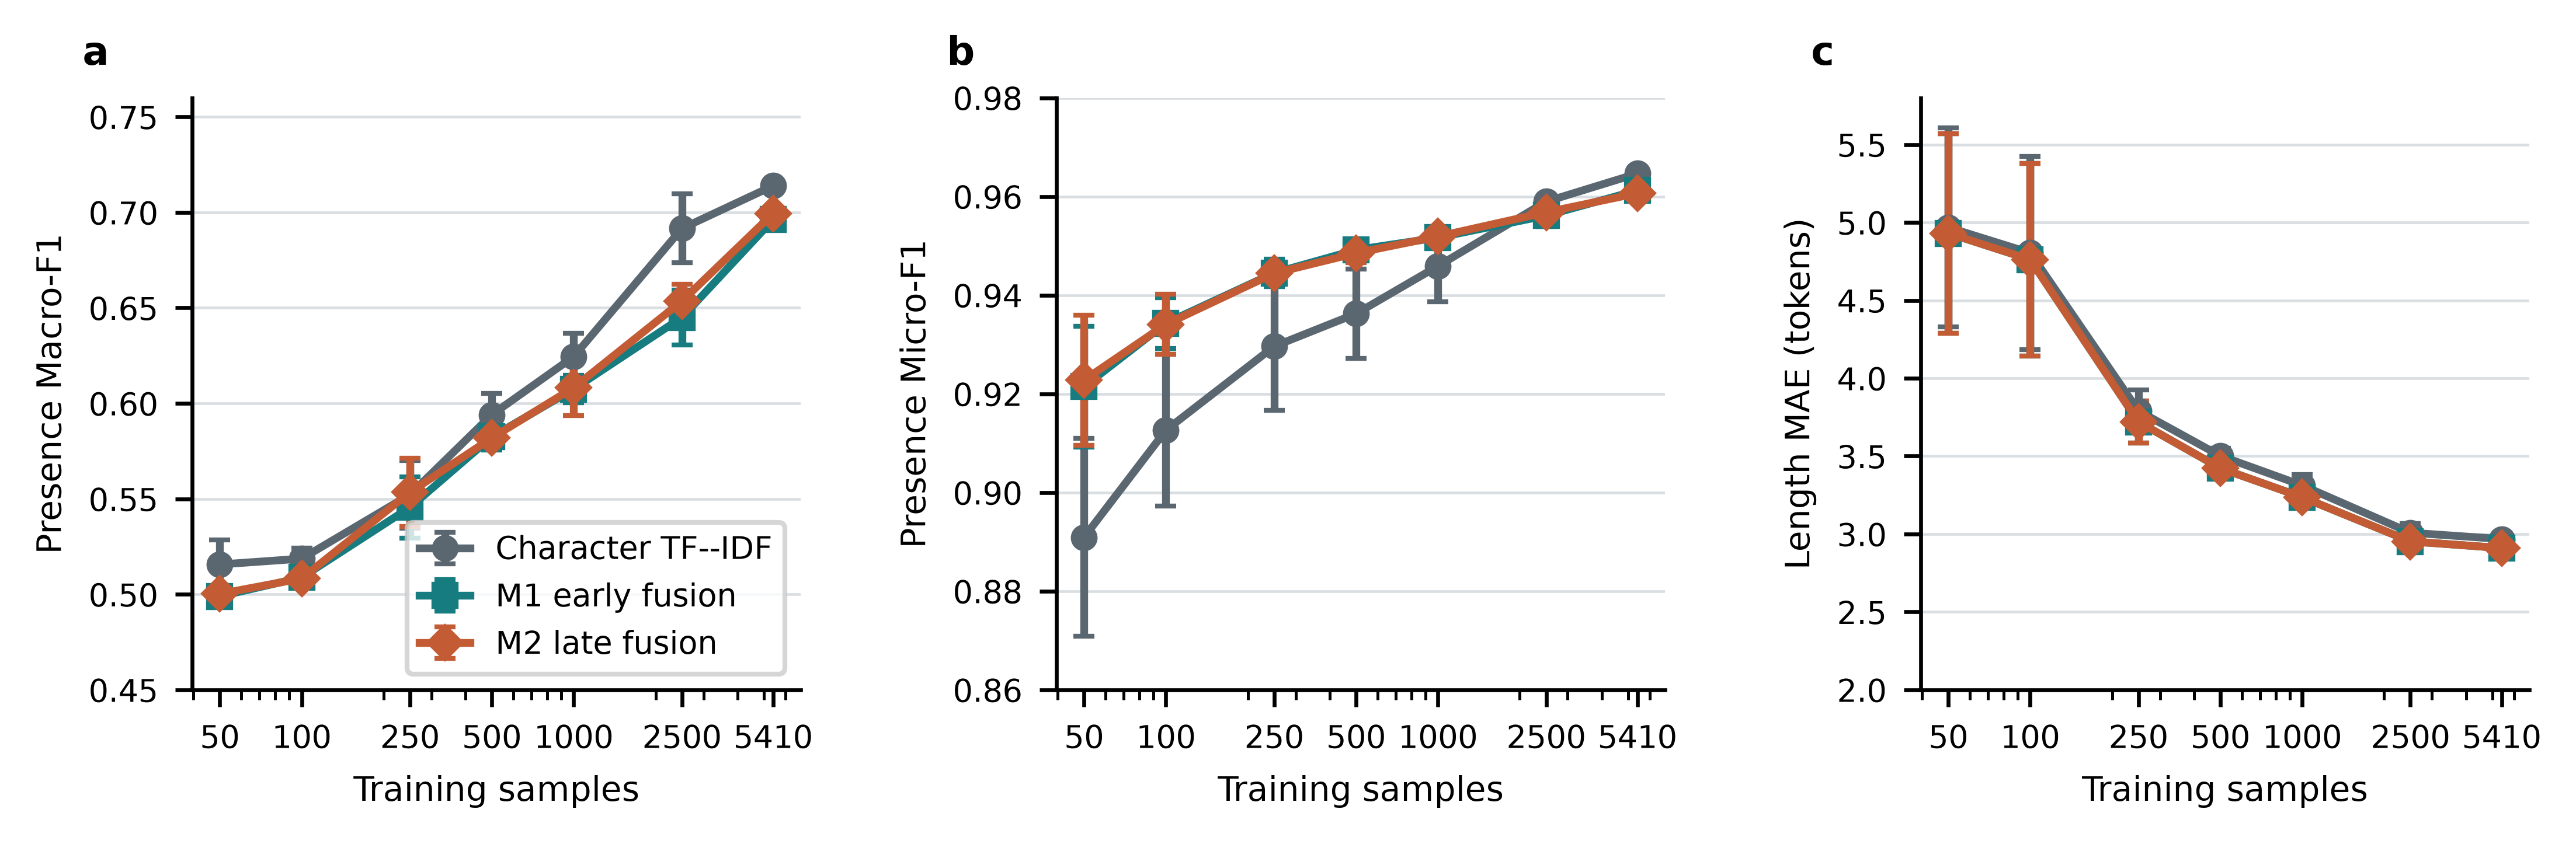
\includegraphics[width=.92\textwidth]{model_strategy_learning_curves.png}
      \captionof{figure}{Offline learning curves for Character TF--IDF, M1 early fusion, and M2 late fusion
 across all training-set sizes. Points and error bars show means and 95\% confidence intervals across five
 random seeds. Character TF--IDF retains higher Macro-F1 at large training sizes, whereas M1 and M2 show
 similar Micro-F1 and length trends. These measures assess FullSchema-derived silver-label selection
 behaviour, not factual extraction accuracy or actual API-token cost.}
\label{fig:offline-main}
\end{center}

随着训练规模从 50 增加到 5410，M1 的 Micro-F1 从 0.9215 增至 0.9612，Length MAE
从 4.9307 降至 2.9100；M2 也从 0.9228 增至 0.9607，Length MAE 从 4.9307 降至 2.9100。
两种融合模型的规模趋势总体接近，但没有显示出稳定的相互优势：在 $n=5410$ 时，M2 的 Macro-F1
为 0.6994，低于 Character TF--IDF 的 0.7139、略高于 M1 的 0.6962；其 Micro-F1 为 0.9607，
接近 M1 的 0.9612，但低于 Character TF--IDF 的 0.9646。因此，后融合没有在当前数据和特征
配置下提供明确的整体收益，在线主实验仍采用 M1。图中的 Length MAE 评价的是由 FullSchema
银标输出构造的长度标签，不是动态 Schema 调用后的完整实测 Token。

图~\ref{fig:offline-budget}考察不同训练规模下，M1 的字段选择行为对完整训练选择结果
的恢复程度。Coverage 表示被选字段对 FullSchema 非空字段的覆盖，Recovery 表示相对于
完整训练模型的恢复；二者均不代表字段值的事实正确性。因此，该图只评估离线选择行为，
不能单独证明真实 LLM 抽取质量。

\begin{center}
\centering
\includegraphics[width=.48\textwidth]{budget_coverage.png}
\includegraphics[width=.48\textwidth]{recovery.png}
\captionof{figure}{Budget coverage and recovery relative to the full model across M1 training-set sizes. Coverage
denotes selected-field coverage of nonempty FullSchema fields, not factual value accuracy; recovery
contextualizes the engineering compromise at $n=100$.}
\label{fig:offline-budget}
\end{center}

图~\ref{fig:offline-budget}中的恢复率进一步说明，小样本首先恢复的是高频字段的
选择行为，宏平均和长度预测的充分恢复需要更多监督。因此 n=100 的选择依据是以较低
启动监督获得可用的字段裁剪，而不是声称它在所有字段上接近完整训练。该图也不能
证明一次性启动训练成本已经被在线工作负载摊销。

\subsection{离线预算回放}

在 6,763 条记录上，预算 100、200 和 400 的平均估计字段成本分别为 90.52、192.67 和
385.04，平均选中字段数为 2.75、4.81 和 8.23，FullSchema 非空字段覆盖率为
26.06\%、53.46\% 和 94.95\%。预算增大确实提高了离线覆盖，但该覆盖率不能替代
重新调用 LLM 后的值质量，也不能直接当作 API 账单。

\section{第二部分：冻结测试集上的 LLM 抽取结果}

离线实验表明，预算约束能够改变字段覆盖范围，但字段被选中并不意味着其值能够被
大语言模型正确抽取。本节因此把问题推进到实际的抽取输出：记录级动态 Schema 能否
在减少总 Token 的同时，保留与模型辅助银标参照的一致性。这里的“保留”并不预设
完整 Schema 是质量上限，而是要求同时观察字段级质量、值级一致性、覆盖范围和调用
负载，判断增加候选字段是否真的转化为可测得的抽取收益。

实验在 500 条冻结评估记录上进行，围绕三个逐层收窄的问题组织证据。第一，字段选择
规则改变的究竟是字段覆盖，还是实际 LLM 输出的质量--Token 权衡；第二，在仅使用
100 条银标启动样本的情况下，主配置是否会因启动样本和模型训练随机性而失稳；第三，
与完整 Schema 及检索式动态 Schema 的比较，能够支持什么范围的工程和方法结论。
Macro-F1 与 Micro-F1 是主要的字段存在性指标，分别用于观察跨字段的均衡表现和总体
实例加权表现；Exact Value Recall、Coverage 与 Total tokens 则用于解释值级一致性、
银标字段覆盖和调用负载之间的取舍。

证据按三个层级展开。首先，在共同成功的记录上进行内部配对比较，以区分完整 Schema、
仅依赖提示词的基线、固定字段诊断和 M1 预算策略的行为；随后在三个随机种子下重复
主配置，以检验有限启动样本条件下的重复性；最后与历史 FullSchema 批次和 SchemaRAG
外部适配实现进行边界对照。字段指标均相对于模型辅助银标参照计算，反映与既有抽取
结果的一致性，而不等同于经过人工核验的事实准确率。在线完成时间和吞吐量不在本节
中推断，而在第三部分的独立性能负载上评价。

\subsection{多种 Schema 策略的内部对照}

正式实验在 500 条冻结评估记录上比较八种方法；所有内部方法使用匹配的模型服务和
调用条件。八种方法的共同成功配对集合为 476 条，因而表~\ref{tab:eight} 的比较重点
是同一批记录上的相对变化，而不是把失败记录差异误归因于字段选择策略。八种方法按
其在实验中的作用分为四组：`full` 提供完整 Schema 的高负载参照；`prompt-null` 和
`prompt-omit` 是仅依赖提示词的基线，用于检验提示词约束本身的作用；`fixed-5` 和
`fixed-10` 使用固定字段先验，仅用于诊断当前数据中高密度字段的上限；`budget-200`、
`budget-400` 和 `lambda=0.003` 则使用 M1 的记录级预测结果进行字段选择，分别考察
硬容量和软成本惩罚下的质量--Token 权衡。表中同时报告字段指标、覆盖率和总 Token，
以避免用单一质量或负载指标决定主方案。

\begin{table}[htbp]
\centering
\scriptsize
\caption{Comparison of eight internal methods on 476 jointly successful records.}
\label{tab:eight}
\begin{tabular}{lccccc}
\toprule
Method & Macro-F1 & Micro-F1 & Exact Recall & Coverage & Total tokens\\
\midrule
full & .7623 & .7410 & .6528 & 1.0000 & 539.83\\
prompt-null & .6215 & .5871 & .6557 & 1.0000 & 548.01\\
prompt-omit & .7475 & .7386 & .6078 & 1.0000 & 487.10\\
fixed-5 (diagnostic) & .8400 & .8382 & .6056 & .7725 & 344.74\\
fixed-10 (diagnostic) & .6633 & .6619 & .6353 & .8409 & 409.39\\
budget-200 & .7759 & .7780 & .6213 & .8303 & 381.49\\
budget-400 & .7736 & .7638 & .6606 & .9763 & 486.32\\
lambda=0.003 & .7822 & .7816 & .6407 & .9606 & 441.28\\
\bottomrule
\end{tabular}
\end{table}

结果首先表明，完整字段集合并不是质量上限。`full` 的字段 F1 并未显示出相对于
动态选择的普遍优势，而 `prompt-null` 在保留完整字段集合的同时具有更低的字段 F1，
说明仅通过空值提示并不能消除额外字段带来的假阳性。换言之，要求模型处理更多字段
会扩大可能的输出范围，但不会自动提高模型对字段存在性的判断。

其次，覆盖率与抽取质量并非单调对应。`budget-400` 的 Coverage 为 0.9763，明显高于
`budget-200` 的 0.8303，但其 Macro-F1 和 Micro-F1 均未提高，同时总 Token 从 381.49
增加到 486.32。这一结果说明，放宽容量主要增加了更多字段的处理负载，也增加了对
低置信度字段进行抽取的机会；Coverage 因而不能作为字段质量的替代指标。

最后，固定字段策略的结果应被解释为数据分布诊断，而不是对记录级选择的否定。`fixed-5`
在当前数据上得到较高的 F1，说明少数高密度字段能够提供一个有用的先验；但这种先验
不使用每条记录的内容差异，无法说明其对稀疏或字段组成不同的记录同样有效。因此，
主方案的选择需要同时考虑字段级质量、银标覆盖和总 Token。基于这一判定，`budget-200`
被作为后续实验的当前折中配置，而不是被解释为在所有数据分布或模型服务上的全局最优。

\subsection{主配置的跨随机种子验证}

在稳定版 Prompt 下，使用 100 条银标启动样本训练的三种 M1 策略均在每个随机种子上
完成全部 500 条记录。这里保持测试记录、LLM 服务、Prompt、字段评价协议和选择规则
不变，仅改变启动样本的随机种子及相应的模型拟合随机性，因此该实验回答的是有限监督
条件下的重复性问题，而不是跨数据分布的泛化问题。`budget-200` 的平均 Macro-F1、
Micro-F1、Exact Value Recall、Coverage 和总 Token 分别为 0.7644、0.7673、0.6470、
0.8381 和 385.5。

提高覆盖程度的 $\lambda=0.003$ 策略和 `budget-400` 分别将平均总 Token 增至 462.2
和 493.2，但没有获得更高的字段级 F1。三种子结果因此提供了两层信息：其一，M1 在
较小启动样本下仍能完成全部冻结记录，说明选择器并非只在单一训练抽样上可运行；其二，
在当前条件下，增加字段预算带来的覆盖扩张没有转化为可测得的整体质量增益。后续实验
采用 `budget-200`，是因为它在这一质量--Token 权衡中提供了较低负载下的稳定折中，
而不是因为三个随机种子足以证明它对所有数据分布或模型服务均最优。三个种子支持的
范围也仅限于当前 Prompt、模型服务、字段集合和银标参照。

\subsection{与完整 Schema 及外部检索策略的边界比较}

与历史完整 Schema 的比较首先提供负载层面的边界证据。新 M1 与历史 FullSchema 并非
同一调用批次；对共同的 476 个 `artifact_id` 进行对齐后，FullSchema 的平均总 Token
为 539.8，M1 `budget-200` 为 385.9，降低约 28.5\%。后者的 Micro-F1 数值更高，但
Exact Value Recall 略低，说明 Token 减少与不同质量指标的变化并不完全同向。这一结果
支持当前配置具有较低 Token 的工程观察，但由于调用批次不同，不能构成严格的显著性
检验，也不能排除批次、服务状态或其他未控制因素的影响。

SchemaRAG 对照考察的是另一种字段选择机制：它根据记录与字段描述的 embedding 相似度
进行固定 Top-$k$ 检索，而 M1 根据字段存在性和长度预测进行预算选择。SchemaRAG k=10
在 500 条完整负载上的 Macro-F1、Micro-F1 和总 Token 分别为 0.7069、0.7022 和 432.9；
k=15 的相应数值为 0.7324、0.7224 和 503.6。M1 `budget-200` 的三种子均值在当前
实现和条件下呈现更高的字段指标与较低的 Token，但该比较同时受到 embedding 模型、
Top-$k$ 设置、缓存和检索开销的影响。SchemaRAG 为依据公开描述完成的外部适配实现，
而非官方方法的严格复现；因此该结果只能限定为当前实现和实验条件下的条件比较，不能
外推为对官方方法或检索式 Schema 选择方法整体的否定。

综合来看，本节支持的结论是：在当前候选字段集合、模型服务、Prompt、有限银标监督和
模型辅助银标评价下，记录级动态 Schema 可以在较低总 Token 下保持具有竞争力的字段级
一致性；这一结论依赖联合观察质量指标与负载指标，并不等同于人工事实准确率，也不构成
跨模型或跨任务的普遍最优性声明。减少字段和 Token 是否进一步转化为端到端完成时间、
有效吞吐和尾延迟收益，需要在不与本节测试集重叠的独立性能负载上单独检验。

\section{第三部分：在线预处理流水线}

\subsection{独立性能负载与实验条件}

性能负载为 2,000 条记录，来自训练集和验证集，不与第二部分测试集重叠。样本按原始
记录字节长度分为五个等频层，每层随机抽取 400 条，随机种子为 20260904。主实验比较
`full`、M1 `budget-200` 和 SchemaRAG k=10，使用 16 个并发消费者和容量为 16 的有界队列，
各重复三次。

\begin{table}[htbp]
\centering
\scriptsize
\setlength{\tabcolsep}{2pt}
\caption{Online-system results on the independent 2,000-record performance workload.}
\label{tab:system}
\begin{tabular}{@{}lccccc@{}}
\toprule
Method & Success rate & Makespan (s) & Effective throughput & Total tokens & P99 (ms)\\
\midrule
full & 100.0\% & 220.82 & 9.06 & 1,709,102 & 3,601\\
budget-200 & 100.0\% & 113.64 & 17.61 & 1,069,254 & 1,308\\
SchemaRAG k=10 & 99.9\% & 399.68 & 5.03 & 1,230,411 & 19,886\\
\bottomrule
\end{tabular}
\end{table}

图~\ref{fig:system-main}检验字段负载缩减是否会传递为端到端在线收益。图比较独立
2,000 条性能负载上的有效吞吐、总 Token、流水线时间和尾延迟；其结论仅适用于当前模型
服务和主要并发端点，不能外推为所有服务或并发配置的缩放规律。

\begin{figure}[htbp]
\centering
\includegraphics[width=.48\textwidth]{main_throughput_and_tokens.png}
\includegraphics[width=.48\textwidth]{main_time_and_tail_latency.png}
\caption{Effective throughput, token workload, pipeline time, and tail latency in the main performance
experiment. The figure tests whether workload reduction transfers to system-level gains; it does not imply
universal scaling across service configurations.}
\label{fig:system-main}
\end{figure}

相对于 `full`，`budget-200` 的在线流水线时间降低 48.54\%，有效吞吐提高 94.38\%，
总 Token 降低 37.44\%。三项指标同时朝有利方向变化，说明在当前条件下字段负载缩减
确实转化为系统级收益，而不是只能从 Token 数字间接推断。相比之下，SchemaRAG 的总
Token 比 `full` 低 28.01\%，但在线 query embedding 累计约 258.61 s，导致整体时间增加
80.99\%，有效吞吐降低 44.43\%。因此，减少 Schema Token 不一定足以抵消额外在线检索
开销，系统比较仍须使用端到端计时。

\subsection{端点方向性验证}

为观察低并发和高并发端点，另在 500 条记录上比较 $c=1,q=1$ 与 $c=32,q=32$，
每种方法和端点重复两次。两种端点同时改变并发度和队列容量，因而不能拆分纯并发
效应与纯队列效应。

\begin{table}[H]
\centering
\scriptsize
\setlength{\tabcolsep}{2pt}
\caption{Endpoint-direction validation; each endpoint changes both $c$ and $q$.}
\label{tab:endpoint}
\begin{tabular}{@{}lcccr@{}}
\toprule
Method & Endpoint & Makespan (s) & Throughput & P99 (ms)\\
\midrule
full & $c=1,q=1$ & 733.49 & 0.68 & 3035\\
budget-200 & $c=1,q=1$ & 463.78 & 1.15 & 1413\\
full & $c=32,q=32$ & 91.04 & 5.49 & 12024\\
budget-200 & $c=32,q=32$ & 33.89 & 14.76 & 2822\\
\bottomrule
\end{tabular}
\end{table}

图~\ref{fig:tradeoff}从两个互补角度检验系统收益是否稳健：左侧比较低、高并发端点的
收益方向，右侧检验较低 Token 是否必然对应较高吞吐。端点图只包含 $c=1,q=1$ 和
$c=32,q=32$，且每个端点同时改变并发度和队列容量；它不是完整并发扫描，也不能分离
并发度与队列容量的独立因果效应。

\begin{figure}[H]
\centering
\includegraphics[width=.48\textwidth]{endpoint_scaling_and_tail_latency.png}
\includegraphics[width=.48\textwidth]{token_throughput_tradeoff.png}
\caption{Endpoint-direction validation and the token--throughput trade-off. The endpoint plot shows
throughput and P99 only at $c=1,q=1$ and $c=32,q=32$; it is not a full concurrency scan and cannot
separate the independent effects of concurrency and queue capacity.}
\label{fig:tradeoff}
\end{figure}

两个端点上，`budget-200` 均表现为更短时间和更高有效吞吐；相对同端点 `full`，低端点
吞吐提高 68.99\%，高端点提高 168.69\%。该结果用于验证收益方向，而高并发端点较高的
尾延迟提示服务端排队和尾部放大。Token--吞吐图进一步显示，`budget-200` 位于较低 Token、
较高吞吐区域；SchemaRAG 虽然比 `full` 少 Token，却因在线 query embedding 和尾延迟开销
具有更低吞吐。因此系统优化不能简化为最小化 Token，仍需同时观察端到端时间、有效成功率
和尾延迟。

\subsection{初始化成本边界与启动成本敏感性分析}

独立初始化实验中，100 条 M1 隔离训练三个 seed 的平均时间为 737.13$\pm$43.69 ms，
模型文件约 3.36 MB；已部署模型冷加载五次平均 178.26$\pm$14.43 ms，P95 为
197.44 ms。100 条 FullSchema 的本地任务规划平均为 366.63 ms，每条 3.09 ms，其中
字段预测约 3.04 ms、Prompt 构造约 0.05 ms。按主实验 FullSchema 的速率换算，100 条
在线推理约 11.04 s，本地规划约占 3.3\%。

这些测量说明本地训练、模型加载和任务规划相对在线 LLM 请求较小，但它们仍是不同的
生命周期阶段。本文不把它们直接加到在线 Token 或 makespan 中。若未来需要全生命周期
成本，可使用：
\begin{equation}
 C_{\mathrm{amortized}}=
 \frac{C_{\mathrm{one-time\ startup}}}{N_{\mathrm{workload}}}
 + C_{\mathrm{online\ per\ record}}.
\end{equation}
当前仅将该式作为成本口径说明，尚未对 100 条启动样本的外部生成成本进行独立现场
计量，也不据此声称全生命周期成本已降低。为检验上述计时边界是否会改变性能判断，
进一步使用已有主实验统计进行离线敏感性
分析。100 条 M1 模型训练和训练后冷加载的保守合计为 0.915 s；已部署模型只需冷加载
时，对应成本约为 0.178 s。主实验的在线时间为 `full` 的 220.82 s 和 M1
`budget-200` 的 113.64 s。若将完整的 0.915 s 保守地只加到 `budget-200` 一侧，
两者分别变为 220.82 s 和 114.56 s，时间差仍为约 106.26 s，因而不会改变领先方向。
这是一种对 M1 不利的不对称假设；实际比较中两种方法共用同一个已训练 M1 模型，训练
和加载成本应视为共享成本，而不应只惩罚动态方法。

进一步按照主实验的有效吞吐，将 100 条记录的在线时间换算为 `full` 约 11.04 s、
`budget-200` 约 5.68 s，每 100 条记录的时间差约 5.36 s。在上述不对称假设下，
0.915 s 的保守启动成本对应约 18 条记录的 break-even；若只计已部署模型冷加载的
0.178 s，则约为 4 条记录。两个数字只用于展示当前测量条件下的一次性成本敏感性，
并不表示公平比较中 M1 实际需要单独回收这些成本，也不适用于其他模型、硬件、服务
 状态或并发配置。

为界定一次性成本的影响范围，图~\ref{fig:initialization-sensitivity} 根据主实验有效吞吐和
已有初始化测量值进行离线敏感性换算，而非新增在线实验。左图比较不同工作负载规模下的累计
时间，右图显示启动成本占 `budget-200` 总时间的比例；0.178 s 和 0.915 s 分别对应已部署模型
冷加载及训练后首次加载的保守假设。

\begin{figure}[htbp]
\centering
\includegraphics[width=.88\textwidth]{initialization_cost_sensitivity.png}
\caption{Sensitivity of the dynamic-Schema performance advantage to one-time initialization costs. Curves
are derived from main-experiment throughput and existing initialization measurements, not new online runs.
The left panel compares `full` with `budget-200` under asymmetric additions of 0.178-s cold-load and
0.915-s train-then-load costs; the right panel shows their shares of total `budget-200` time. Approximately
4 and 18 records are the corresponding break-even estimates. Both methods share the trained M1 model in
the actual comparison, so the figure does not assign these costs exclusively to the dynamic method.}
\label{fig:initialization-sensitivity}
\end{figure}

该敏感性分析显示，启动成本主要影响极小工作负载；随着记录数增加，在线吞吐差异成为累计
时间的主要决定因素。约 4 条和 18 条记录的 break-even 分别对应两种假设，且只说明当前测量
条件下的一次性成本边界，不构成完整生命周期成本审计。

该分析还确认，100 条 `full` 任务的本地 Producer 规划总计 0.367 s，其中 M1
字段预测约 3.04 ms/条、Prompt 构造约 0.05 ms/条；这些时间已经包含在 Runner 的
在线 Producer 阶段，不能再次加到既有在线流水线时间上。初始化分析不包含环境安装、
容器启动、数据库冷缓存或多进程重复加载，因此不构成完整生命周期成本审计。

\section{讨论}

本文的中心发现有两个层次。首先，少量 FullSchema 银标监督足以训练一个在真实 LLM
调用中可用的字段选择器；但离线 Macro-F1 和长尾字段结果表明，这种“小样本可用性”
不是对所有字段的均衡识别能力。其次，动态 Schema 的 Token 减少在当前单进程流水线
中确实伴随更短 makespan 和更高有效吞吐，说明字段裁剪改变了在线工作负载，而不是只
改变离线成本估计。

预算实验还揭示了一个重要的反例：更高字段覆盖率并不自动带来更高端到端质量或更好
系统性能。`lambda` 和 `budget-400` 保留了更多字段，却产生更多输出 Token；SchemaRAG
虽然减少了部分 Token，却因在线 embedding 成本和尾延迟降低了整体吞吐。因此，方法
评价需要同时观察字段质量、Token、服务时间、重试和尾延迟。

当前结论有以下限制：
\begin{enumerate}
  \item 监督和参考结果来自 model-assisted silver reference，不是独立人工 Gold；
  \item 当前 API 价格未配置，`actual_cost` 不应解释为免费或真实货币成本下降；
  \item 新 M1 与历史 FullSchema 的 aligned476 结果来自不同调用批次，只能描述性比较；
  \item SchemaRAG 是基于论文描述的外部重实现；
  \item 系统是单进程异步有界流水线，性能负载为 2,000 条记录，端点实验同时改变 $c$ 和 $q$，不能给出队列容量
        或并发度的独立因果结论；
  \item 本文未在数十万条或生产规模记录上进行端到端验证，因此文化遗产数据仅构成当前
        方法的评估场景，不能据此宣称已验证大规模部署能力；
  \item 在线性能不含启动样本生成、银标构造、训练和模型加载的一次性成本；现有离线
        敏感性分析显示，保守地计入 0.915 s 后性能领先方向不变，但这不是完整生命周期
        成本审计。
\end{enumerate}

后续工作可补充独立人工或证据验证集；如需完整生命周期成本结论，还应补测启动样本生成、环境和部署阶段的成本。系统方面，可在固定 $c$ 下进行 $q$ 消融，并在
单进程结果稳定后研究多进程分片和协调器；这些工作不能用当前结果预先替代。

\section{结论}

本文提出并实证分析了一个由少量 FullSchema 银标监督驱动的预算感知动态 Schema 选择
流程。M1 n=100 的 `budget-200` 在 500 条冻结记录上保持了稳定的字段级指标，同时
将在线 Token 负载压低；在独立 2,000 条性能负载、16 个并发消费者和容量为 16 的有界队列条件下，该负载缩减
对应 48.54\% 的流水线时间下降和 94.38\% 的有效吞吐提升。该结果支持这样一个
受限判断：对于信息密度不均的记录集合，记录级 Schema 裁剪可以成为 LLM 预处理流水
线的有效负载整形机制。

这一判断仅适用于当前模型服务、Prompt、数据集和单进程实现。一次性启动成本的完整摊销、
队列容量独立效应以及多进程或多节点扩展，均应作为后续证据，而
不是当前结论的一部分。

\section*{数据、代码与结果来源}

训练数据、划分、模型和评估报告位于项目目录
`/root/work/papers/extraction/`。主要结果目录为：
\begin{itemize}
  \item `reports/model_strategy_ablation/` 与 `reports/training_size_ablation/`；
  \item `reports/quality_token_comparison.*`；
  \item `benchmarks/analysis/performance/`。
\end{itemize}
在线运行入口为 `llm_runner.py`，性能统计和绘图入口分别为
\path{benchmarks/analyze_performance_results.py} 与
\path{benchmarks/plot_performance_figures.py}。
所有图表均从已固化的离线 CSV 或报告生成，未在本文稿编译过程中发起 LLM 或 Embedding
调用。

\section*{相关工作与参考文献}

\subsection*{LLM 结构化信息抽取}
ChatSchema [1] 将 Schema 引导的分类与结构化键值抽取结合起来，说明大语言模型可以依据
预定义字段生成结构化结果。UIE [8] 将实体、关系和事件等任务统一为结构化预测问题，
InstructUIE [9] 进一步通过指令微调支持多种信息抽取任务；InstructGPT [7] 则代表了
instruction-following 模型遵循复杂任务指令的基础发展。上述工作通常假设目标 Schema
已经确定，并在抽取时直接提供完整字段集合。本文关注其前置问题：对于一条具体记录，
是否需要在调用 LLM 前暴露全部候选字段。

\subsection*{动态 Schema 与 Schema 优化}
SchemaRAG [2] 根据输入记录与 Schema 元数据之间的语义相似度检索相关字段，再将固定
Top-$k$ 字段交给 LLM，以减少上下文和输出负载。本文采用少量完整 Schema 抽取产生的
模型辅助银标训练记录级字段预测器，并将字段效用、估计字段成本和预算约束共同纳入
选择。本文的 SchemaRAG 对照依据公开描述完成，是只实现 query--field Top-$k$ 检索的
外部适配实现，不是官方代码复现。

PARSE [3] 将 JSON Schema 视为面向 LLM 的自然语言 contract，并通过自动优化和约束
机制改善结构化抽取过程；Schema-adaptable Knowledge Graph Construction [4] 关注知识
图谱 Schema 随任务或时间变化时的适应。前者优化 Schema 的定义与表达，后者处理全局
Schema 的演化，而本文假设候选字段集合相对稳定，研究记录级字段子集的调用前选择。

\subsection*{预算感知抽取与 Prompt 压缩}
Doctopus [5] 从数据管理角度研究预算感知的结构化抽取，根据预估资源开销在不同抽取
方案之间进行选择。本文将这一决策粒度推进到记录条件下的 Schema 字段，并在 LLM 调用
前执行轻量字段裁剪。FrugalGPT [10] 通过模型路由、级联和自适应模型选择控制调用
开销；本文不进行模型路由，而是在同一 LLM 服务前进行字段级选择。LLMLingua [11]
通过压缩 Prompt 中的冗余 Token 降低推理负载；本文的操作对象不是连续文本 Token，
而是具有明确语义和任务权重的 Schema 字段。

\subsection*{LLM serving 与文化遗产应用}
PagedAttention [6] 代表了从推理服务内部优化 LLM 吞吐的工作，通过更高效的 KV-cache
管理支持高并发服务。本文的 Producer--Consumer 流水线不改动 KV-cache 或服务引擎，
而是测量字段裁剪如何改变请求负载、端到端完成时间、有效吞吐和尾延迟，因此与
serving 系统优化互为补充。Huang 等 [12] 使用知识图谱和深度学习支持数字文化遗产
管理，说明结构化文化遗产信息具有明确的应用背景。本文将文化遗产记录作为具体评估
场景，考察结构化抽取前的记录级字段选择；该文献不作为本文方法有效性、生产规模或
跨数据集结论的证据。

\begin{enumerate}[label={\arabic*}.]
  \item Fei Wang, Yuewen Zheng, Qin Li, Jingyi Wu, Pengfei Li, Luxia Zhang. ChatSchema:
        A Pipeline of Extracting Structured Information with Large Multimodal Models Based
        on Schema. arXiv preprint arXiv:2407.18716, 2024.
  \item Sin Yu Bonnie Ho, Arlie Coles, Erik Larsson, Eric Marshall, Nathan Bodenstab, Paul
        Vozila. SchemaRAG: Dynamic Large Schema Reduction for LLM-driven Structured
        Information Extraction. In Proceedings of the 64th Annual Meeting of the Association
        for Computational Linguistics, Industry Track, 1114--1127, 2026. DOI:
        10.18653/v1/2026.acl-industry.78.
  \item Anubhav Shrimal, Aryan Jain, Soumyajit Chowdhury, Promod Yenigalla. PARSE: LLM
        Driven Schema Optimization for Reliable Entity Extraction. In Proceedings of the
        2025 Conference on Empirical Methods in Natural Language Processing, Industry
        Track, 2749--2763, 2025. DOI: 10.18653/v1/2025.emnlp-industry.184.
  \item Hongbin Ye, Honghao Gui, Xin Xu, Xi Chen, Huajun Chen, Ningyu Zhang.
        Schema-adaptable Knowledge Graph Construction. arXiv preprint arXiv:2305.08703, 2023.
  \item Yuanhao Zhong, Yuhao Deng, Chengliang Chai, Ruixin Gu, et al. Doctopus: A System for
        Budget-aware Structural Data Extraction from Unstructured Documents. In
        SIGMOD-Companion 2025, 275--278, 2025. DOI: 10.1145/3722212.3725103.
  \item Woosuk Kwon, Zhuohan Li, Siyuan Zhuang, Ying Sheng, Lianmin Zheng, Cody Hao Yu,
        Joseph E. Gonzalez, Hao Zhang, Ion Stoica. Efficient Memory Management for Large
        Language Model Serving with PagedAttention. In Proceedings of the 18th USENIX
        Symposium on Operating Systems Design and Implementation, 973--990, 2024.
  \item Long Ouyang, Jeffrey Wu, Xu Jiang, Diogo Almeida, Carroll Wainwright, Pamela
        Mishkin, Chong Zhang, Sandhini Agarwal, Katarina Slama, Alex Ray, John Schulman,
        Jacob Hilton, Frans Oleg, Ryan Lowe, et al. Training Language Models to Follow
        Instructions with Human Feedback. In Advances in Neural Information Processing
        Systems, 2022.
  \item Yao Lu, Qin Chen, Zhe Li, Dongsheng Cai, Zhiqiang Zhang, Xiaodong Zhang. UIE:
        Universal Information Extraction as Structured Prediction. In Proceedings of the
        60th Annual Meeting of the Association for Computational Linguistics, 507--519,
        2022.
  \item Yujie Wang, Yucheng Li, et al. InstructUIE: Multi-task Instruction Tuning for
        Universal Information Extraction. arXiv preprint arXiv:2304.08085, 2023.
  \item Lingjiao Chen, Matei Zaharia, James Zou. FrugalGPT: How to Use Large Language Models
        While Reducing Cost and Improving Performance. Transactions on Machine Learning
        Research, 2024.
  \item Huiqiang Jiang, Qianhui Wu, Chin-Yew Lin, Yuqing Yang, Lili Qiu. LLMLingua:
        Compressing Prompts for Accelerated Inference of Large Language Models. In
        Proceedings of the 2023 Conference on Empirical Methods in Natural Language
        Processing, 13358--13376, 2023. DOI: 10.18653/v1/2023.emnlp-main.825.
  \item Yuexin Huang, Suihuai Yu, Jianjie Chu, Hao Fan, Bin Du. Using Knowledge Graphs and
        Deep Learning Algorithms to Enhance Digital Cultural Heritage Management. npj
        Heritage Science, 11:204, 2023. DOI: 10.1186/s40494-023-01052-6.
\end{enumerate}

\end{document}
